\section{Statistics}\label{section:statistics}

Robust predictive modeling and statistical inference are crucial for successful analyses in particle physics.
This section will be a very brief tour of these concepts and some of their applications, which will be necessary to understand the analysis that was performed.

\subsection{Likelihood Ratio}\label{section:likelihood_ratio}

\subsubsection{Wilk's Theorem}\label{subsection:wilks_theorem}

In brief, Wilk's theorem~\cite{Wilks:1938dza} states that for two functions in a nested family of functions, $f\left(x\,\middle|\,\vec{\theta}_{a}\right)$ and $f\left(x\,\middle|\,\vec{\theta}_{b}\right)$, with the number of parameters $a < b$, in the limit of large sample size the likelihood ratio test statistic,
\begin{equation}
 t_{\vec{\theta}} = -2 \log \frac{\displaystyle L\left(\vec{\theta}_{a}\right)}{\displaystyle L\left(\vec{\theta}_{b}\right)},
\end{equation}
is asymptotically distributed as a $\chi^2$ random variable with $d=b-a$ degrees of freedom,
\begin{equation}
 f\left(t_{\vec{\theta}} \,\middle|\,\vec{\theta}\, \right) \to \chi^2_{d}.\label{eq:wilks_theorem}
\end{equation}
This asymptotic approximation to the empirical distribution of the test statistic allows for efficient computation of a \pvalue{} (that approximates the \pvalue{} under the empirical distribution).

The one-sided (one-tailed) \pvalue{} --- given the null hypothesis that $t_{\vec{\theta}}$ is $\chi_{d}^{2}$ distributed --- is then the value of the complementary cumulative distribution function (CCDF) of the $\chi^2_{d}$ distribution evaluated at the observed $t_{\vec{\theta}}$,
\begin{equation}
 p\textrm{-value} = \textrm{CCDF}_{\chi^2_{d}}\left(x=t_{\vec{\theta}}\right).
\end{equation}
That is to say, the \pvalue{} is the probability, given $t_{\vec{\theta}} \sim \chi^2_{d}$, to observe a $t_{\vec{\theta}}$ value greater than or equal to that which was observed.

\subsubsection{Profile Likelihood Ratio}

The \gls{MLE} $\hat{\theta}$ is the value of the parameter $\theta$ that maximizes the likelihood function given the observed data.
So for parameter of interest $\mu$ and nuisance parameters $\vec{\theta}$, the maximum likelihood estimators are $\hat{\mu}$ and $\hat{\vec{\theta}}$.
Likewise, the conditional maximum likelihood estimator $\hat{\hat{\theta}}$ is the value of the parameter $\theta$ that maximizes the likelihood for a given value of another parameter $\mu$.
So for a specific value of the parameter of interest $\mu$, the conditional maximum likelihood estimator for nuisance parameters $\vec{\theta}$ is $\hat{\hat{\vec{\theta}}}$.
As $\hat{\hat{\vec{\theta}}}$ is a function of the given $\mu$ then it is seen that the likelihood function's dependence on the nuisance parameters $\vec{\theta}$ can be ``profiled'' vs. $\mu$ and removed.
Given this, the profile likelihood ratio,
\begin{equation}
 \lambda\left(\mu\right) = \frac{L\left(\mu, \hat{\hat{\vec{\theta}}}\right)}{L\left(\hat{\mu}, \hat{\vec{\theta}}\right)}\,,
 \label{eq:profile_likelihood_ratio}
\end{equation}
can be constructed and used as a test statistic to indicate the compatibility of a possible value $\mu$ with the MLE $\hat{\mu}$ --- a function of the observed data.
Given that the negative log likelihood is usually what is actually calculated --- for numerical reasons --- the test statistic that is generally used from the profile likelihood ratio is
\begin{equation}
 q_{\mu} = -2 \ln \lambda\left(\mu\right) = 2 \left(\ln L\left(\hat{\mu}, \hat{\vec{\theta}}\right) - \ln L\left(\mu, \hat{\hat{\vec{\theta}}}\right)\right)\,,
 \label{eq:q_mu}
\end{equation}
as it is seen by Wilk's theorem, \Cref{eq:wilks_theorem}, to be distributed according to a $\chi^{2}$ distribution with one degree of freedom.
This results in a \pvalue{} for $q_{\mu}$ of
\begin{equation}
 p = \int\limits_{q_{\mu}}^{\infty} f_{\chi^{2}}\left(t\middle|1\right)\,dt\,.
 \label{eq:q_mu_pvalue}
\end{equation}

\subsection{Intervals and limits}\label{section:intervals_and_limits}

In addition to point estimates that determine an estimator, $\hat{\theta}$, of a parameter $\theta$, interval estimates give statistical precision to the measured value.
A common example of such an interval estimate is the set of points bounded by the point estimate and the estimated standard deviation: $\left[\hat{\theta} - \sigma_{\hat{\theta}}, \hat{\theta} + \sigma_{\hat{\theta}}\right]$.
The following is a short discussion of the construction, interpretation, and use of these intervals in the frequentist and Bayesian paradigms.

\subsubsection{Frequentist Confidence Intervals}

In the frequentist paradigm, a $1-\alpha$ confidence level (CL) confidence interval (CI) is an interval estimate that covers the true value of the parameter, $\theta$, $1-\alpha$ of the time it is constructed.
So the $95\%$ confidence level confidence interval covers the true value $95\%$ of the time it is constructed.
The method for constructing confidence intervals is called the ``Neyman Construction''~\cite{Neyman:1937uhy}, and results from inverting hypothesis tests.
This confidence interval construction can be described as a random variable that is the set of parameter points, $\left\{\vec{\theta}\right\}$, where the null hypothesis of each parameter point $\theta$ is accepted, $p\left(t > k_{\alpha}\middle| \theta\right) < \alpha$,

\begin{equation}
 \mathrm{CI}_{1-\alpha} = \left\{\vec{\theta}\,\middle| \,p\left(t > k_{\alpha}\middle| \vec{\theta}\right) < \alpha\right\}\,.
 \label{eq:confidence_interval}
\end{equation}

By construction, a hypothesis test of size $\alpha$ should accept the null hypothesis, given that the null is true, $(1-\alpha)$ of the time~\cite{Cranmer:2015nia}.

It is very important to take care in interpreting the meaning of the confidence interval, as it is often misunderstood and misused in analysis.
The confidence interval is constructed from the observed data%
\footnote{The data are a random variable in the frequentist paradigm.}
and so is a random variable and reflects information regarding the constructed estimator --- not the true parameter.
The confidence interval does \emph{not} give the interval in which there is a $1-\alpha$ probability of finding the true parameter value.
This is manifestly Bayesian and in fact is the interpretation of a Bayesian credible interval.
Keeping the definition of frequentist probability tightly in mind, the confidence interval should be interpreted as an interval of parameter values that $1-\alpha$ \emph{of the times is constructed} contains the true parameter value.
Given this, in the frequentist paradigm one is \emph{unable} to make any statement on the probability that the true parameter value is contained in any specific confidence interval beyond the tautology that the true parameter is either contained in it or it is not.
Any misuse of this result is not from a failing of the paradigm, but a misplaced desire of the analyst to have different questions answered than were asked.

In terms of computing a confidence interval, from observations that are governed by $\theta$ a test statistic, $t$, that is an estimator of $\theta$ is constructed.
For each value of the parameter to be tested, there exists an interval $\left[t_{1}, t_{2}\right]$ such that the probability of $t \in \left[t_{1}, t_{2}\right]$ is
\begin{equation}
 p\left(t_{1} < t < t_{2}\middle|\theta\right) = \int\limits_{t_{1}}^{t_{2}} f\left(t\middle|\,\theta\right)\,dt = 1-\alpha\,.
 \label{eq:confidence_interval_coverage}
\end{equation}
This interval represents a constant line segment in the $\left(t, \theta\right)$ parameter space plane at the given value of $\theta$.
By repeating this procedure for every value of $\theta$ to be tested, a band of line segments --- a ``confidence belt'' --- is created that is bound between the curves $\theta\left(t_{1}\right)$ and $\theta\left(t_{2}\right)$, as shown in the example in \Cref{fig:confidence_belt}.
Then, for any given observed value of the test statistic, $t'$, a boundary at $t = t'$ can be drawn in the plane that intersects the confidence belt at the points $\left(t', \theta_{2}\right)$ and $\left(t', \theta_{1}\right)$.
This resulting range of parameter values $\left[\theta_{1}, \theta_{2}\right]$ is the confidence interval~\cite{Cranmer:2015nia,PDG2018:Ch39}.

\begin{figure}[htbp]
 \centering
 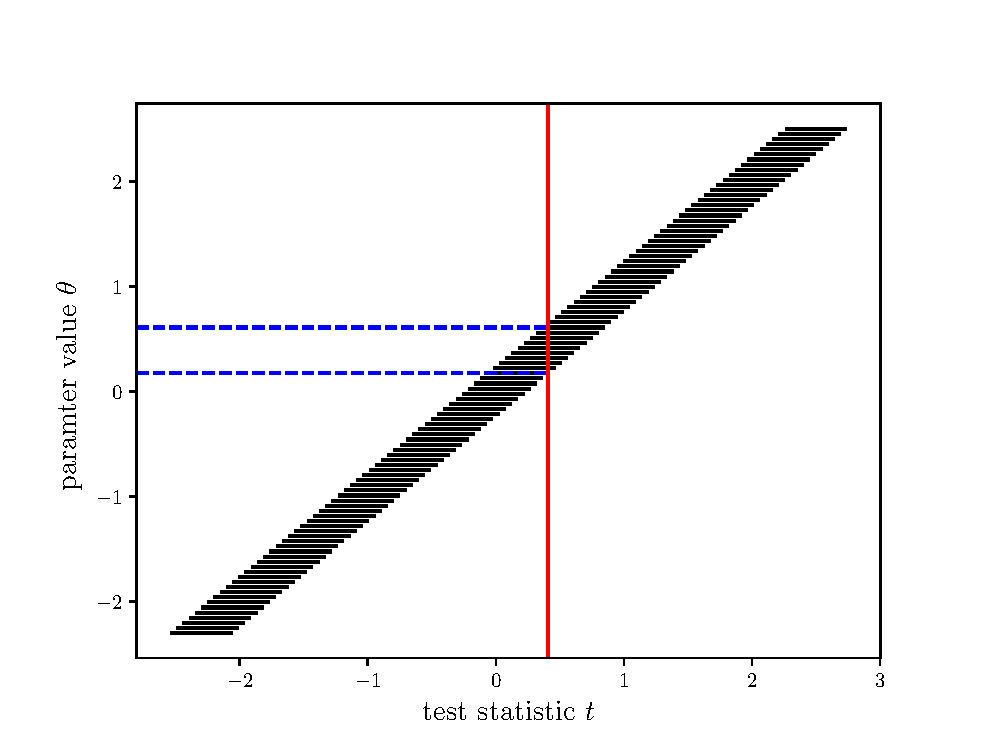
\includegraphics[width=0.6\linewidth]{preface/confidence_belt.eps}
 \caption[Neyman construction of a confidence interval using a confidence belt.]{%
  Example sketch of the construction of a confidence belt showing an observation in red intersecting the belt and the corresponding confidence interval as the parameter values bounded between the two blue dashed lines.}\label{fig:confidence_belt}
\end{figure}

The conditions of coverage from \Cref{eq:confidence_interval_coverage} do not uniquely specify $t_{1}$ and $t_{2}$, which allows for analysis specific choices to be made.
If central intervals are chosen, then the probabilities excluded below $t_{1}$ and $t_{2}$ are both $\alpha/2$.
In the event that only an upper (or lower) limit is of interest, as is common in searches for new physics where no excess has been observed, then the probability excluded below $t_{1}$ (or above $t_{2}$) is zero.
Alternatively, if the test statistic used is the profile likelihood ratio test statistic,
\[
 q_{\theta} = -2 \ln\lambda\left(\theta\right) = -2 \ln\frac{L\left(\theta, \hat{\hat{\phi}}\,\right)}{L\left(\hat{\theta},\hat{\phi}\right)}\,,
\]
profiling determines the allowed range $\left[q_{\theta, 1}, q_{\theta, 2}\right]$.
It is seen from \Cref{eq:q_mu} and \Cref{eq:q_mu_pvalue} that for an observed $q_{\theta}$, $q_{\mathrm{obs}}$, to satisfy \Cref{eq:confidence_interval} the resulting confidence belt are the values $q_{\theta} < q_{\mathrm{obs}}$, and the resulting confidence interval the range of $\theta$ that enforce this.
Using such a test statistic results in the Feldman-Cousins confidence intervals~\cite{Feldman:1997qc}.

As the confidence interval can be a difficult concept to describe, a simple illustrative example follows.
Consider $n$ observations $\vec{x} = \left\{x_{1}, \cdots, x_{n}\right\}$ that are drawn from a Normal distribution with unknown mean $\theta$ and width $\sigma_{\theta}$.
This results in a sample mean $\hat{\theta}$ and standard deviation $\sigma_{\hat{\theta}}$.
To construct a $95\%$ confidence level central confidence interval for $\theta$, the test statistic $t = \left(\hat{\theta} - \theta\right)/\sigma_{\hat{\theta}}$ can be used such that ${p\left(t_{1} < t < t_{2}\middle|\theta\right) = 0.95}$, where $t_{1}$ and $t_{2}$ are respectively the $2.5$th percentile and $97.5$th percentile%
\footnote{$t_{1} = \mathrm{CDF}^{-1}\left(\alpha/2\right)$ and $t_{2} = \mathrm{CDF}^{-1}\left(1 - \alpha/2\right)$.}
of the Student's $t$-distribution for $n-1$ degrees of freedom, mean $\mu=\hat{\theta}$ and standard deviation $\sigma=\sigma_{\hat{\theta}}$.
Transforming the Student's $t$-distribution by $t' = \left(t-\hat{\theta}\right)/\sigma_{\hat{\theta}}$ to have $\mu=0, \sigma=1$ simplifies to ${p\left(-d < t' < d\middle|\theta\right) = 0.95}$.
Transforming to parameter space, ${p\left(\hat{\theta} - d\, \sigma_{\hat{\theta}} < \theta < \hat{\theta} + d\, \sigma_{\hat{\theta}}\right)  = 0.95}$, this gives a confidence interval of $\left[\hat{\theta} - d\, \sigma_{\hat{\theta}}, \hat{\theta} + d\, \sigma_{\hat{\theta}}\right]$.
Confidence intervals following this example construction are simulated and shown in \Cref{fig:confidence_intervals}.

\begin{figure}[htbp]
 \centering
 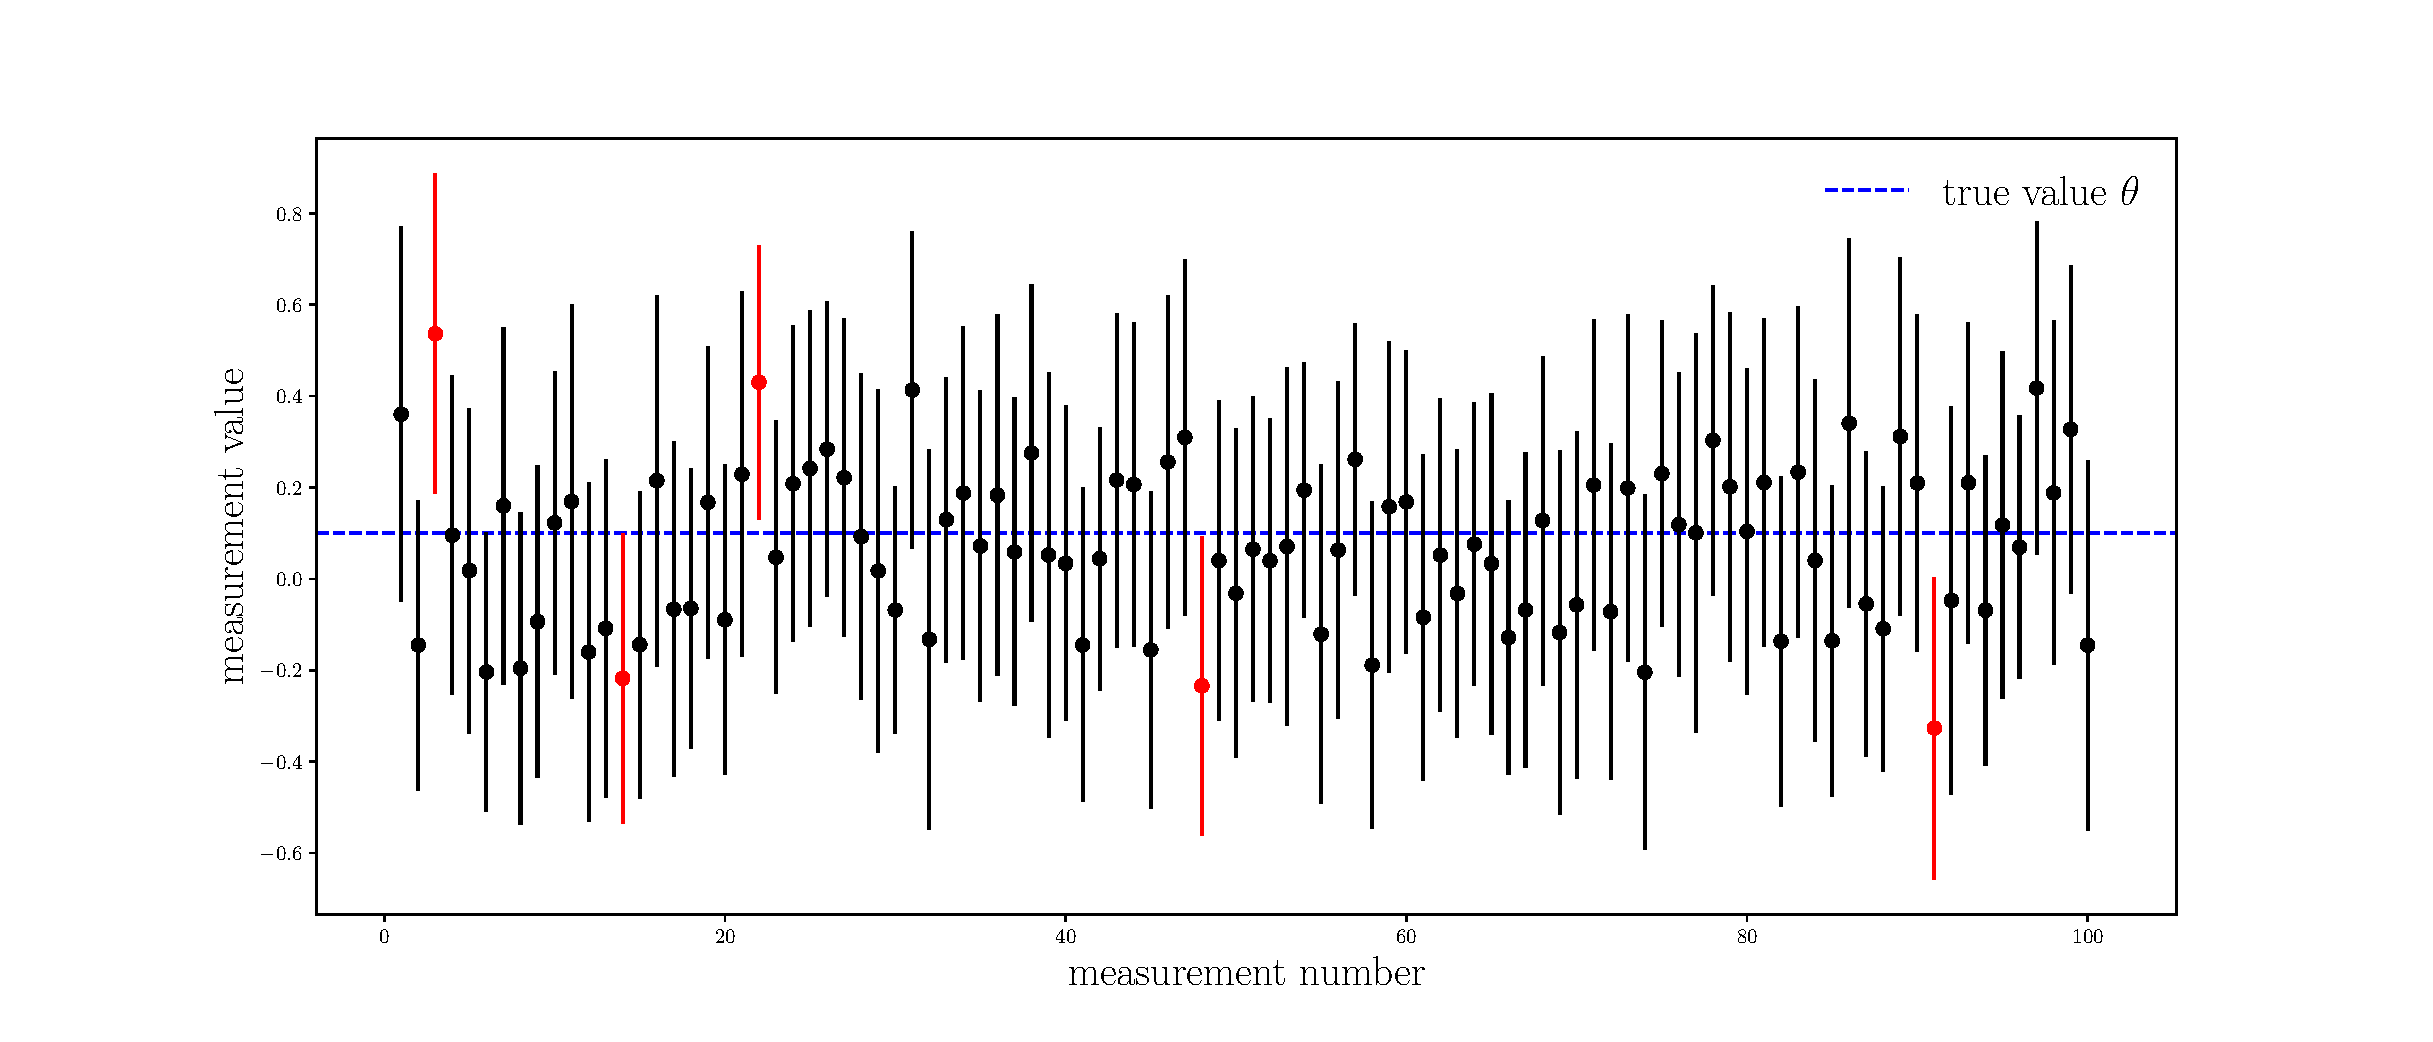
\includegraphics[width=\linewidth]{preface/confidence_intervals.eps}
 \caption[Simulation of 100 $95\%$ confidence level confidence intervals]{%
  An example of 100 point estimates and associated $95\%$ confidence level confidence intervals of parameter value $\theta$.
  Each measurement is the result of the same number of samples from a Normal distribution.
  Confidence intervals that do not include the true value $\theta$ (dashed blue line) are colored red.}
 \label{fig:confidence_intervals}
\end{figure}

\subsubsection{Bayesian Credible Intervals}

In the Bayesian paradigm, a $1-\alpha$ credibility level (CL) credible interval (CI)%
\footnote{CL and CI are used for abbreviations for both the frequentist and Bayesian intervals.
 It will be made clear to the reader from context which paradigm is being considered.}
is an interval estimate where there is a $1-\alpha$ probability of containing the true parameter value --- which is a random variable.
As a result, it is simply the interval of the posterior predictive distribution $\left[\theta_{1}, \theta_{2}\right]$ that when integrated over gives a probability of $1-\alpha$,

\begin{equation}
 p\left(\theta_{1} < \theta < \theta_{2}\middle|\vec{x}\right) = \int\limits_{\theta_{1}}^{\theta_{2}} p\left(\theta\middle|\,\vec{x}\right)\,d\theta = 1-\alpha\,.
 \label{eq:credible_interval_coverage}
\end{equation}

As in the frequentist paradigm, there are different ways to select the credible interval range.
One can choose the shortest interval,%
\footnote{For a unimodal distribution this interval is known as the highest posterior density interval (HPD).}
the interval where probabilities excluded below $\theta_{1}$ and above $\theta_{2}$ are both $\alpha/2$ (this interval includes the median), the interval centered at the mean of the posterior (if the mean exists), or the intervals corresponding to upper (or lower) limits which reduce \Cref{eq:credible_interval_coverage} to the CDF (or CCDF) of $\theta$.

As a final word on interval estimates, it is worth remembering that the frequentist and Bayesian paradigms address different questions and so make different statements with their intervals.
\begin{itemize}
 \item Frequentist: When a confidence interval is constructed on future data, the constructed interval will contain the true parameter value with a probability (frequency) of $1-\alpha$.
 \item Bayesian: Given the observed data, there is a $1-\alpha$ probability that the true parameter value is contained by the constructed credible interval.
\end{itemize}
